\documentclass[12pt, a4paper, simple]{eskdtext}

\usepackage{hyperref}
\usepackage{env}
\usepackage{_sty/gpi_lst}
\usepackage{_sty/gpi_toc}
\usepackage{_sty/gpi_t}
\usepackage{_sty/gpi_p}
\usepackage{_sty/gpi_u}

% Код
% \ESKDletter{О}{Л}{Р}
% \def \gpiDocTypeNum {81}
% \def \gpiDocVer {00}
% \def \gpiCode {\ESKDtheLetterI\ESKDtheLetterII\ESKDtheLetterIII.\gpiStudentGroupName\gpiStudentGroupNum.\gpiStudentCard-0\gpiDocNum~\gpiDocTypeNum~\gpiDocVer}

\def \gpiDocTopic {ОТЧЁТ ЛАБОРАТОРНОЙ РАБОТЫ №\gpiDocNum}

% Графа 1 (наименование изделия/документа)
% \ESKDcolumnI {\ESKDfontII \gpiTopic \\ \gpiDocTopic}

% Графа 2 (обозначение документа)
% \ESKDsignature {\gpiCode}

% Графа 9 (наименование или различительный индекс предприятия) задает команда
% \ESKDcolumnIX {\gpiDepartment}

% Графа 11 (фамилии лиц, подписывающих документ) задают команды
% \ESKDcolumnXIfI {\gpiStudentSurname}
% \ESKDcolumnXIfII {\gpiTeacherSurname}
% \ESKDcolumnXIfV {\gpiTeacherSurname}

\begin{document}
    \begin{ESKDtitlePage}
    \ESKDstyle{empty}
    \begin{center}
        \gpiMinEdu \\
        \gpiEdu \\
        \gpiKaf \\
    \end{center}

    \vfill

    \begin{center}
        \gpiTopic
    \end{center}

    \vfill

    \begin{center}
        \textbf{\gpiDocTopic} \\
        ПО ДИСЦИПЛИНЕ \gpiDiscipline \\
    \end{center}

    \vfill

    \begin{flushright}
        \begin{minipage}[t]{7cm}
            Выполнил:\\
            \PageTitleStudentInfo
            \PageTitleDateField
            \hspace{0pt}

            Проверил:\\
            \PageTitleTeacherInfo
            \PageTitleDateField
        \end{minipage}
    \end{flushright}

    \vfill

    \begin{center}
        \PageTitleCity~\ESKDtheYear
    \end{center}
\end{ESKDtitlePage}

    \ESKDstyle{empty}
    %
    \textbf{Цель лабораторной работы}: Изучение основ разработки интерфейсов мобильных приложений.

    Задачи лабораторной работы:
    \begin{itemize}
        \item Изучить элементы интерфейса.
        \item Практическим путём научиться размещать элементы и менять их свойства.
        \item Разработать прототип интерфейса собственного приложения.
    \end{itemize}

    \subparagraph{Разработка дизайна} \hspace{0pt}

    \begin{figure}[!h]
        \centering
        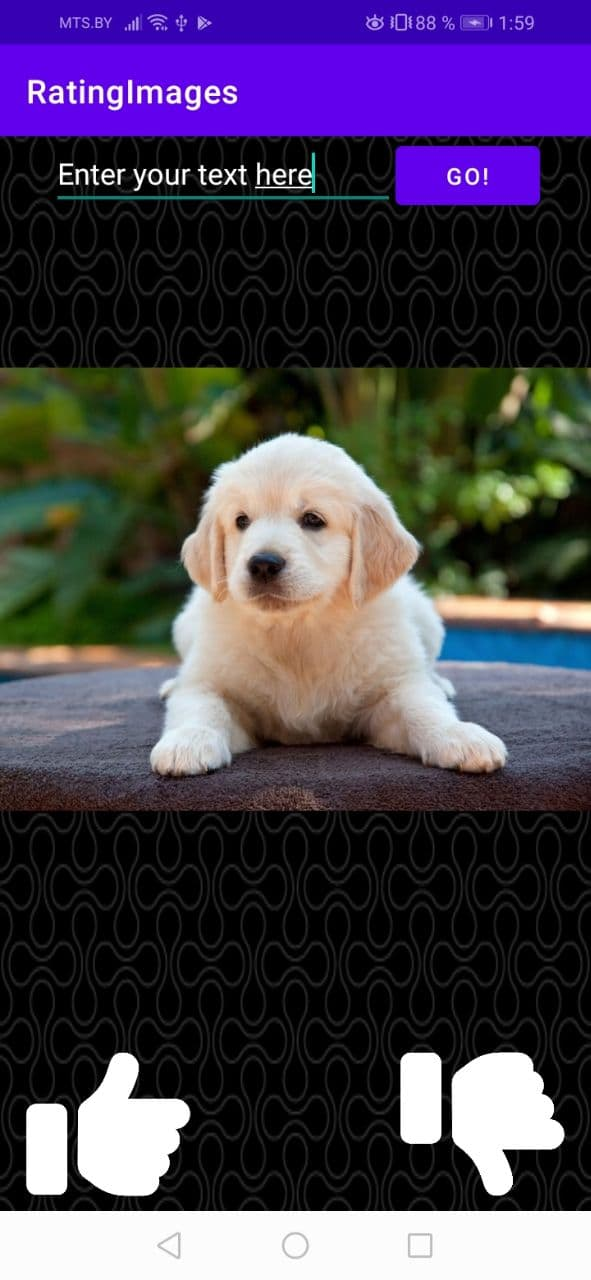
\includegraphics[height=11cm]
            {_assets/gpi_RaitingImages.jpg}
        \caption{Приложение <<RaitingImages>>}
        \label{fig:gpi_hit}
    \end{figure}

    \lstinputlisting[language=xml, name=app/src/main/res/values/strings.xml]
        {../gpi_src/gpi_rpodms6_lab3/app/src/main/res/values/strings.xml}

    \lstinputlisting[language=xml, name=app/src/main/res/drawable/backgroud.xml]
        {../gpi_src/gpi_rpodms6_lab3/app/src/main/res/drawable/backgroud.xml}

    \lstinputlisting[language=xml, name=app/src/main/res/layout/activity_main.xml]
        {../gpi_src/gpi_rpodms6_lab3/app/src/main/res/layout/activity_main.xml}

    % \lstinputlisting[language=java, name=app/src/main/java/.../gpi_rpodms6_lab2/MainActivity.java]
        % {../gpi_src/gpi_rpodms6_lab2/app/src/main/java/io/github/Pavel_Innokentevich_Galanin/gpi_rpodms6_lab2/MainActivity.java}

    \subparagraph{} \hspace{0pt}

    \textbf{Вывод}: Разработал дизайн приложения <<RaitingImages>>.
    Использовали LinearLayout, RelativeLayout и FrameLayout для слоев.
    Задали верхнему тегу задний фон.
    Создали EditText с текстом подсказкой, занеся в string.xml. Поменяли цвет EditText.
    Создали кнопку Button c текстом из string.xml.
    Создали ImageView, указан ссылку на картинку и contentDescription.

    \newpage

    \section*{Список использованных источников}
    \addcontentsline{toc}{section}{Список использованных источников}

    \begin{enumerate}
        \item[1.] Кондратюк, А. П.
        Разработка приложений для мобильных операционных систем «Android» : ЭУМК для
        студ. второй ступени (магистратуры) специальности 1-31 81 06 <<Веб-программирование и интернет-технологии>>
        физ.-мат. фак. / А.П. Кондратюк ; Брест. гос. ун-т им. А.С. Пушкина, каф. ПМиИ. – Брест : электрон. издание БрГУ, 2016. – 469 с.\\
        §20. Лабораторная работа №3 cс.~298-347

        \item[2.] Как исправить ошибку в android studio? — Хабр Q8A
        - [Электронный ресурс]. Режим доступа:
        URL: \url{https://qna.habr.com/q/575266}.
        (Дата обращения: 16.02.2022).

        \item[3.] java - This view is not constrained - Stack Overflow
        - [Электронный ресурс]. Режим доступа:
        URL: \url{https://stackoverflow.com/questions/37817537/this-view-is-not-constrained}.
        (Дата обращения: 16.02.2022).

        \item[4.] SpaceRequiredBeforeStandalone - XMLdation Wiki
        - [Электронный ресурс]. Режим доступа:
        URL: \url{https://wiki.xmldation.com/Support/Validator/SpaceRequiredBeforeStandalone}.
        (Дата обращения: 16.02.2022).

        \item[5.] Subtle Patterns | Free textures for your next web project
        - [Электронный ресурс]. Режим доступа:
        URL: \url{https://www.toptal.com/designers/subtlepatterns/}.
        (Дата обращения: 16.02.2022).

        \item[6.] android - Failed to get GED Log Buf, err(0) - Stack Overflow
        - [Электронный ресурс]. Режим доступа:
        URL: \url{https://stackoverflow.com/questions/50158481/failed-to-get-ged-log-buf-err0}.
        (Дата обращения: 16.02.2022).

        \item[7.] puppy: 2 тыс изображений найдено в Яндекс.Картинках
        - [Электронный ресурс]. Режим доступа:
        URL: \url{https://yandex.by/images/search?pos=0&from=tabbar&img_url=https%3A%2F%2Fpbs.twimg.com%2Fmedia%2FDlCjT7xXgAI4L2u.jpg&text=puppy&rpt=simage}.
        (Дата обращения: 16.02.2022).

        \item[8.] Font Awesome
        - [Электронный ресурс]. Режим доступа:
        URL: \url{https://fontawesome.com/search?q=like&s=solid%2Cbrands}.
        (Дата обращения: 16.02.2022).

        \item[9.] Font Awesome
        - [Электронный ресурс]. Режим доступа:
        URL: \url{https://fontawesome.com/icons/thumbs-down?s=solid}.
        (Дата обращения: 16.02.2022).

        \item[10.] SVG to PNG – Convert SVG files to PNG Online
        - [Электронный ресурс]. Режим доступа:
        URL: \url{https://svgtopng.com/}.
        (Дата обращения: 16.02.2022).

        \item[11.] Post-Download Page | Krita
        - [Электронный ресурс]. Режим доступа:
        URL: \url{https://krita.org/en/post-download-page/}.
        (Дата обращения: 16.02.2022).
        
    \end{enumerate}
\end{document}
